
\begin{figure*}[t]
  \centering
  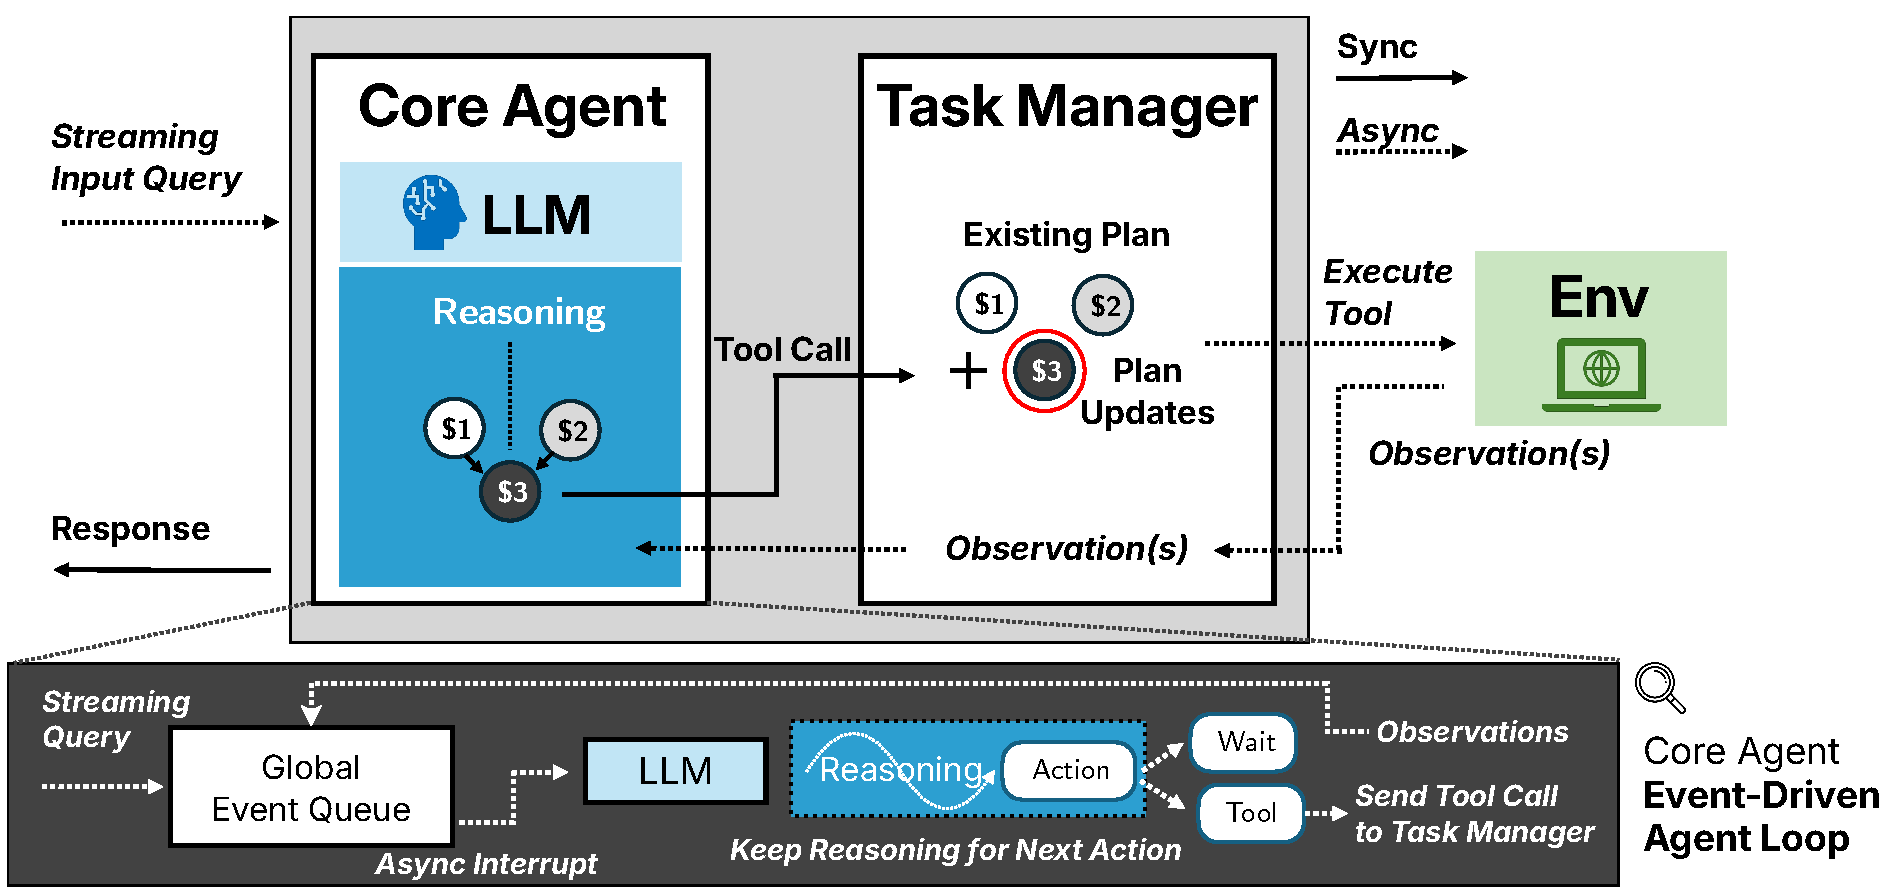
\includegraphics[width=0.9\textwidth]{figures/rta_sys_diagram.pdf}
  % \vspace{-7mm}
  % \vspace{-5mm}
  \caption{
  \textbf{Top:} Architecture diagram for our system implementation, which consists of: i) a core agent loop that receives streaming user inputs and tool responses from the environment and which launches tool calls as needed; and ii) a task manager that manages in-flight tool calls and tracks dependencies.
\textbf{Bottom:} A zoomed-in diagram showing the core event-driven control loop, which injects new information from the user and environment into the model's context as it arrives.
The model is allowed to reason and act continuously while waiting for additional information. 
  }
  % \vspace{-3mm}
  \label{fig:system-architecture}
\end{figure*}

\section{Method}

\subsection{Asynchronous I/O}
\label{sec:asynchronous-io}

The aim of our methodology is to enable models to reason and act continuously while waiting on information from either the user or the environment. 
Building on prior work on LLM agent processing based on partial inputs for voice agents ~\citep{arora2025stream,chiang2025shanks,shih2025can}, as well as prior work on asynchronous tool use ~\citep{gim2024asynchronous}, we propose \textit{Asynchronous Input/Output (I/O)}, where we decouple the agent's thinking and acting stream from information coming from the user as well as information arriving from tool execution. 
This decoupling allows the model to work continuously while waiting for additional information from the user or from the environment.

We assume that the user input is provided incrementally as it is available, with updates provided in ``$<partial\_query\_update>$'' / ``$</partial\_query\_update>$'' tags (and with ``$<final\_query\_update>$'' / ``$</final\_query\_update>$'' used to denote the end of utterance from the user).
To enable Asynchronous I/O, we design a set of possible actions to enable the model to think and act asynchronously with respect to the user and environment.
At each step, the model must first produce reasoning (encompassed in ``$<think>$'' / ``$</think>$'' tags), and then produce one of the following actions:
\begin{enumerate}
    \item ``$<tool\_call> ID. tool\_name(a1, a2, ...)</tool\_call>$'' to call tool $toolname$ with arguments $a1, a2, ...$ (where $ID.$ is an integer starting from 1 that denotes the tool call ID, and which is used to label the tool call observation, which is returned asynchronously as ``$<information> ID. ...</information>$'')
    \item ``$<pause>$'' to halt generation and wait for more information from the user or environment if there is no other action required based on currently available information
    \item ``$<answer> ... </answer>$'' to produce the final answer
\end{enumerate}

The tool call IDs are used for tracking and editing tool calls before they are finalized (see Sec. \ref{sec:spec-tool-calling}).
When additional information from the user or environment becomes available while the model is generating, we halt the model's generation and inject the updated information (with ``$</think\_interrupted>$'' prepended to the information).

Additionally, there are forbidden cases which we must consider: i) the model should not pause for information if there are no outstanding tool calls and it has already received the final user update, ii) the model should not produce the final answer before receiving the full user query, and iii) cases where there are formatting errors with the generation or action.
For all these cases, instead of processing the invalid action, we inject an error message instructing the model to not repeat this behavior and we restart generation.
Section \ref{sec:inference-framework} describes how our system implementation injects information into the model's context when updates arrive from the user and environment. 

\subsection{Speculative Tool Calling}
\label{sec:spec-tool-calling}

Our system aims to launch tool calls as soon as enough information is received from the user or environment to reduce latency. However, there are multiple challenges with launching tool calls based on partial information from the user or environment:

\begin{enumerate}
    \item Even if we know that a tool call is required, we may not yet have received all the information from the environment required to call the tool (e.g. we know that we need to send a message to a given contact, but we are still waiting on an earlier tool call to retrieve the contact information).
    \item It is possible that additional information arrives from the user (or from tool observations) which \emph{invalidates} a tool call which was generated based on partial information, and we need to modify or remove the tool call.
    \item Additionally, not all tool calls can be launched speculatively, as some tool calls modify the system state irreversibly.
\end{enumerate}

In our work, we aim to address these challenges to enable asynchronous reasoning and acting with respect to the user/environment while ensuring correct execution of tool calls.
Our approach builds on the approach from LLMCompiler~\citep{kim2024llm} by managing tool calls as a Directed Acyclic Graph (DAG). 
The existing LLMCompiler method addresses challenge 1) by allowing for emitting tool calls which depend on previous (not yet executed) tool calls. 

To address challenges 2) and 3), we propose \textit{Speculative Tool Calling}, which enables launching tool calls early and later refining tool calls based on updated information from the user or environment.
This approach is visualized in Figure \ref{fig:execution-trace}.
To deal with the challenge that particular ``write'' tools cannot be executed until we are certain that we have received all of the required information (since they irreversibly modify system state), we manually classify tools as either safe or unsafe to execute speculatively based on whether the tool has any side effects (i.e., tools that only read information are marked as safe, whereas tools that modify system state are marked as unsafe), and then hold up execution for unsafe tools until a final confirmation signal is received.
This approach is inspired by how speculative read and write operations are handled in computer hardware memory systems, where write operations are buffered but not allowed to execute until the instruction is committed~\citep{yeager2002mips}. 
Note that this approach still allows for overlapping reasoning and selecting the action while waiting for additional information, so it still reduces latency for tools which are not safe to execute speculatively.

To allow the model to edit tool calls which have already been produced but have not yet been executed, we allow the model to either \textit{modify} or \textit{remove} existing tool calls that have already been issued.
To \textit{modify} a tool call, the model needs to generate a tool call with the same ID as the one that it wants to overwrite (see Sec. \ref{sec:asynchronous-io}).
To \textit{remove} a tool call, the model instead generates a special tool call ``$REMOVE$ $ID.$'', which cancels the tool call with the provided ID.
For tool calls which have executed speculatively and which are later invalidated, if the observation has not yet been inserted into the model's context, we discard it.
When discarding observations, we inject a cancellation message encapsulated in $<cancel>$ / $</cancel>$ tags to inform the model not to expect information to be inserted as
``$<information> ID. ...</information>$''.
If there were any tool calls which depended on the output of the cancelled tool call, these are also cancelled.
For tool calls which are not safe to execute speculatively, if these are modified or removed, the invalid tool call is never executed.
Additionally, to help the model understand which tool calls are active, we provide plan hints each time it produces a tool call or receives a query update (providing the current active tool calls in 
``$<current\_plan>$'' / ``$</current\_plan>$'' tags).

For tools that are not safe to execute speculatively, we allow them to begin execution at the \textit{commit} point.
The \textit{commit} point occurs when the following conditions are met: i) the final query update has been received, and ii) the model either generates a tool call ID greater than any previously generated (implying that any edits to the existing tool calls is complete) or generates a pause action (indicating that there are no other modifications required to the existing plan).
At this point, all tool calls that were held up because they were unsafe to execute speculatively begin execution once all of their dependencies are satisfied.

\subsection{Inference Framework}
\label{sec:inference-framework}

\label{sec:training}

\begin{figure*}[t]
  \centering
  % \includegraphics[width=0.85\textwidth]{figures/training-diagram.pdf}
  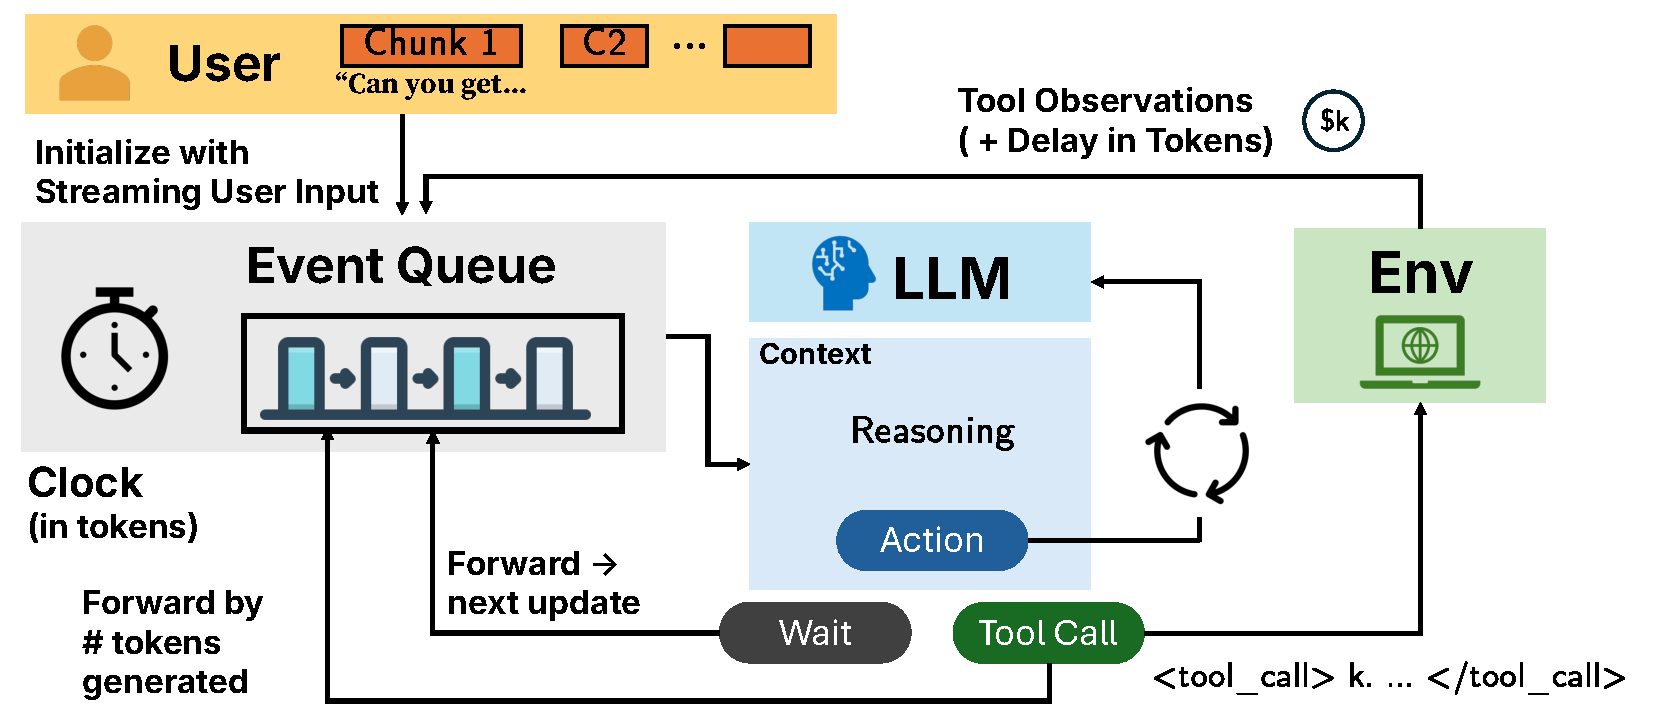
\includegraphics[width=0.85\textwidth]{figures/rta_training_sys.pdf}
  % \vspace{-7mm}
  \caption{
  \textbf{Training Infrastructure.} A diagram showing how our training infrastructure works to adapt the model to reason and act while waiting on delayed inputs from the user and environment.
  We use an environment which runs on a ``clock'' (with time kept in terms of number of tokens to generate before the model would receive the update). 
  Our approach maintains a central update queue which buffers events until they are ready and then interrupts the model and injects the information into the model's context.
  The model is allowed to reason and act continuously while waiting for additional updates.
  }
  \label{fig:train-system}
  % \vspace{-3mm}
\end{figure*}

We present a system implementation to enable the model to reason and act asynchronously with respect to the user and environment, as well as tracking information to manage speculative tool execution.
As described in Figure \ref{fig:system-architecture}, our system is decoupled into a core agentic loop and a task execution manager.
The core agentic loop uses an event-driven framework as in~\citep{rllm2025pepper}. 
At each timestep, the model is allowed to reason and act iteratively based on the currently available information, and it can also wait if no more work can be done until additional information is provided.
When additional information is provided by the user or returned from tool execution, this information can be immediately injected as a new event into a global event queue, and it can then be injected into the model's context.
The core LLM loop uses interruptible streaming with vLLM ~\citep{kwon2023efficient} so that interrupts can be injected immediately as they return.


As in prior work \citep{kim2024llm}, our system leverages a tool execution task manager to launch tool calls as they are ready. 
The manager supports dependency tracking as in \citep{kim2024llm}, which enables launching tool calls which depend on previous tool calls that have not yet finished execution, and which also allows tool calls to execute in parallel if they do not depend on one another.
Similar to \citep{gim2024asynchronous}, as tool calls finish execution, the results can be injected immediately into the context of the model.
Different from these prior efforts, our task manager supports iteratively adding new tasks to the task manager, as well as correcting or removing tool calls from the task queue if later user/environment updates invalidate the earlier tool calls.
Additionally, our task manager also tracks whether tools are safe to execute speculatively, and holds up unsafe tools until the final commit signal is provided.

